\chapter{Motor Imagery: the hunt for a greek letter}
\label{chapter:five}
\epigraph{...utilizing the brain signals in man-computer dialogue.}{Vidal}

\section{Introduction}

Motor Imagery is an EEG or ECoG based BCI paradigm originated on changes of SMR, sensorimotor rhythms, that are altered when a person engages in motor behavior, but it can also be elicited when a person imagines to perform any movement. Particularly, the Rolandic wicket rhythm, the $\mu$ rhythm, is of the same frequency (e.g. 8-12 Hz) of visual occipital alpha waves, but from a spatially different location (posterior frontal and anterior parietal areas)\cite{WolpawJonathanR2012}.   Although SMR patterns presents a high inter- and intra-subjects variability regarding the signal features required to identify them, an Event Related Desynchronization/Synchronization of $\mu$ rhythm is in general consistent across subjects, regardless of the specificity of the imagined movement (i.e. what is being imagined to move).

\section{Materials and Methods}

In order to verify if this ERD/ERS could be detected by the method presented in this work, i.e. by automatically extracting the information from the signal plots, a BCI Simulation was performed against the public Motor Imagery Dataset 002-2014, published by BNCI-Horizon 2020 website and initiative~\cite{Steyrl2015}.  This dataset is composed of 8 runs for 14 participants.  The first 5 runs were used for training without feedback, and the remaining 3 runs were used to test the results.  The original online experiment was performed with 20 trials on each run, 10 corresponding to imagining moving the right hand and the other 10 to feet movement.  Figure~\ref{fig:midatasetdiagram} schematize the protocol and the structure of the published dataset.  This BCI simulation experiment was divided in two.  In the first simulation, baseline signals, corresponding to the 1st second of each trial were compared against right hand motor imagery, 4.5 seconds ahead of the beginning of each trial. Signal segments of 1s length were processed for 10 trials for each of 5 runs and their descriptors extracted for both classes.  The second BCI simulation was similar but only extracting trials corresponding to feet movement imagery.

\begin{story}[BCI Simulation or Cross Validation?]
The decoding part of BCI Research inherits practices from Machine Learning and a cross-validation procedure is a common practice.  However, in terms of the data extracted from the brain of a person who is learning and changing how to perform a certain operation does not make too much sense to use information from a future brain to derive outputs in the past.

The idea of implementing a BCI Simulation is not very well defined in BCI research, but their practice without naming it has been the regular approach for BCI Competitions. The idea is to use an offline dataset simulating what would have happened if the system has been tested in real-time following the same sequence of operations that what was used to generate the dataset.

Regardless, of any definition, the Online Validation with feedback of any BCI system is the Gold Standard due to Man-Machine Dilemma.
\end{story}


\begin{figure}[]
\centering
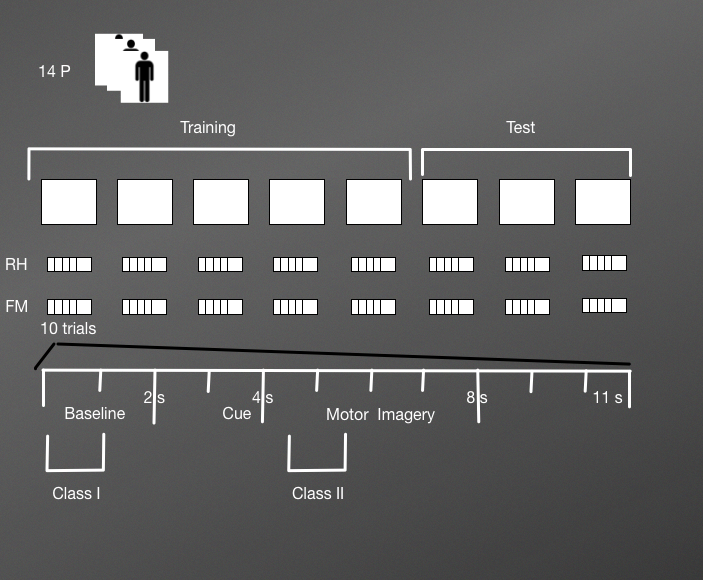
\includegraphics[scale=0.6]{images/DatasetIIIDiagram2.png}
\caption[Motor Imagery Experimental Protocol]{Fourteen voluntary Participants performed 5 sessions of training and 3 sessions of testing.  On each session each subject had 10 trials to perform Right Hand Motor Imagery and 10 trials for Feet Movement.  At the same time, each trial has a 2-seconds baseline and a 4-seconds section to perform the imagery task.  For each BCI Simulation, Class 1 is defined from EEG information obtained from the baseline section, while Class 2 is based on extracting segments from the imagery section of the EEG signal.}
\label{fig:midatasetdiagram}
\end{figure}


\section{Results}

Binary classification accuracies are calculated based on the output of the BCI simulation on the remaining 3 runs for each participant, in a single-trial approach: for each sampled segment of 1-second length, classification based on the classification algorithm described in \ref{nbnn} is applied and a match or mismatch is obtained.  Results are shown in Figure~\ref{fig:miresults} where for right-hand detection \textit{RH}, average accuracies of around $70\%$ are obtained for the channel C3, the best-performing channel, coincidentally with the contralateral structure of the imagined movement.  On the other hand, the binary classification accuracy for feet imagery detection \textit{FM}, achieves in all the channels accuracies of just above chance level.

%TODO Theoretical chance level from the NAM book of lotte.
   
\begin{figure}[h!]
\centering
\subfigure[]
{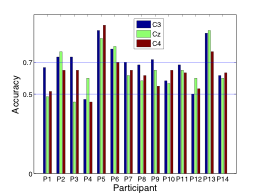
\includegraphics[width=7cm, height=5cm]{images/MIinformedonpaper1.png}}
\subfigure[]
{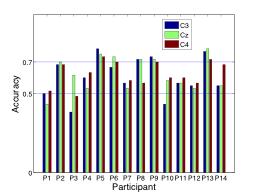
\includegraphics[width=7cm, height=5cm]{images/MIinformedonpaper2.png}}
\caption[Motor Imagery Accuracy]{Classification Accuracy for discriminating segments of 1s ($\gls{N} = 512$) of EEG for Motor Imagery detection BCI simulation. (a) Accuracy values for channels C3, Cz and C4 for the 14 participants of the described MI dataset discriminating between baseline and right-hand imagery. (b)The same procedure for feet imagery. Accuracy levels averaged to $70\%$ are obtained only for right-hand movement on the contralateral channel C3. The SIFT descriptor size for this dataset was adjusted to 72x72 pixels}.
\label{fig:miresults}
\end{figure}
   
\section{Conclusion}

Offline BCI Simulation of single trial asynchronous triggering for right hand MI based on signal plots was implemented with a level of success of 70\% for 7 out of 14 Participants. Single trial asynchronous triggering of BCI can be implemented with this paradigm, particularly for right-hand motor imagery. The name $\mu$ rhythm was precisely coined because the shape of the waves have some resemblance to the greek letter~\cite{Cole2017}.   Additionally, in line with previous chapter results, the frequency of these components is exactly the same as alpha waves, 10 Hz.

% Parameters
% Poner una figura donde más o menos se vean las señales.


